% -*- root: ../InvestigacionOperativa.tex -*-

Vamos a definir unos conceptos para poder hacer unas observaciones pertinentes al ejemplo resuelto (estos conceptos serán utilizados a lo largo del curso).


\begin{defn}[Solución\IS factible]
Cualquier punto que verifique todas las restricciones se llama solución factible.
\end{defn}

\begin{defn}[Conjunto\IS factible]
El conjunto factible es el conjunto de todas las soluciones factibles (en el dominio de la función objetivo).
\end{defn}

\begin{defn}[Solución\IS factible óptima]
La solución factible óptima es la solución factible para la que se optimiza el objetivo.
\end{defn}

\begin{defn}[Problema\IS lineal]
Un problema de optimización es lineal si tanto la función objetivo como las funciones que definen las restricciones son lineales.
\end{defn}


\paragraph{Observaciones sobre el problema de la intruducción (\ref{prob:intro})}
\begin{itemize}
	\item Este problema que hemos resuelto es un problema lineal, en el que además el conjunto factible es convexo (un poliedro).
	\item Además, la solución coincide con uno de los vértices del conjunto factible.
	\subitem En algún momento del curso veremos que siempre hay un vértice que es solución de un problema.
	\item El vértice está definido por 2 restricciones que se satisfacen con igualdad (saturadas o activas en ese punto).
	\item Un problema lineal puede tener una solución factible óptima única, puede tener infinitas soluciones o puede no tener solución.
	\subitem En este problema tendríamos infinitas soluciones si la recta de nivel fuera paralela a alguna de las fronteras. En ese caso, toda la frontera sería solución.
	\subitem 
\end{itemize}

Vamos a ver 3 ejemplos resolviéndolos gráficamente. Uno con una única solución (también en un vértice) otro con infinitas soluciones y un último ejemplo sin ninguna solución óptima.

\begin{example}
Estudiamos el siguiente problema:

\begin{ioprob}
\goal{$\max 2x_1 + x_2$}
\restrictions{$X_1 + 3x_2 \leq 2$}{$x_1,x_2\geq 0$}{}{}{}{}
\end{ioprob}

\begin{center}
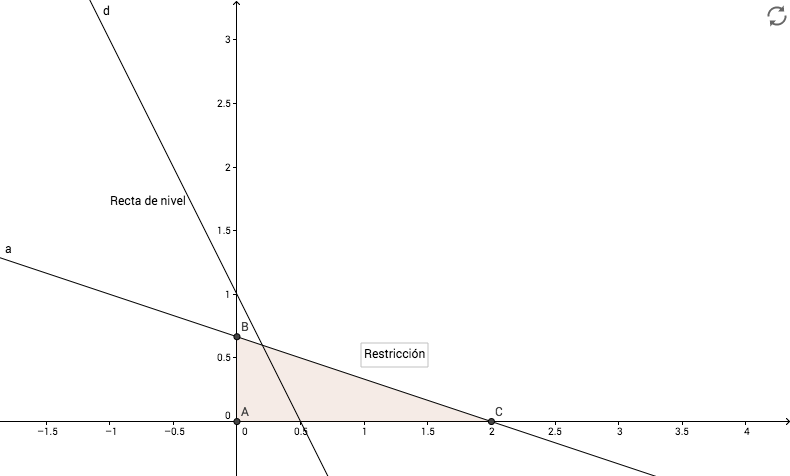
\includegraphics[scale=0.45]{img/io-intro_1.png}
\end{center}

Este problema tiene solución factible óptima única. Si desplazamos la recta de nivel en la dirección perpendicular, llegamos a la intersección con $C$.
\end{example}

\begin{example}
Estudiamos el siguiente problema:

\begin{ioprob} 
\goal{$z = 2x_1+x_2$}
\restrictions{$x_1+2x_2 \leq 2$}{$x_1,x_2\geq 0$}{}{}{}{}
\end{ioprob}


\begin{center}
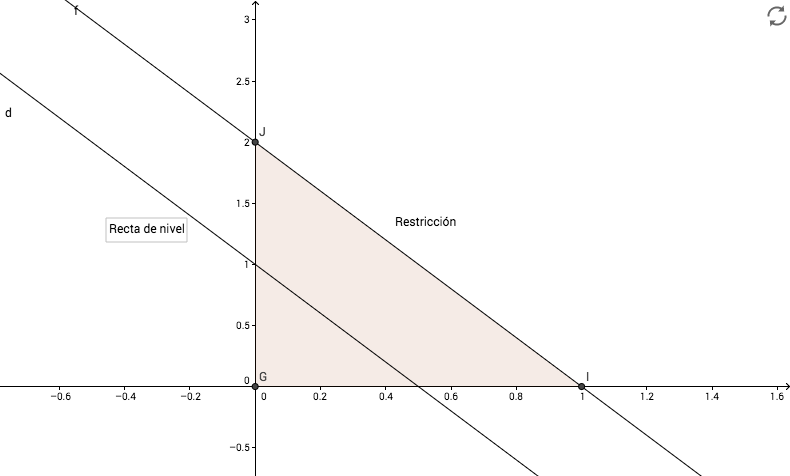
\includegraphics[scale=0.45]{img/io-intro_2.png}
\end{center}


Este problema tiene infinitas soluciones óptimas.
\end{example}

\begin{example}

Estudiamos el siguiente problema:

\begin{ioprob} 
\goal{$2x_1 + x_2$}
\restrictions{$-x_1+x_2\leq 1$}{$x_2\leq 3$}{$x_1,x_2\geq 0$}{}{}{}
\end{ioprob}

\begin{center}
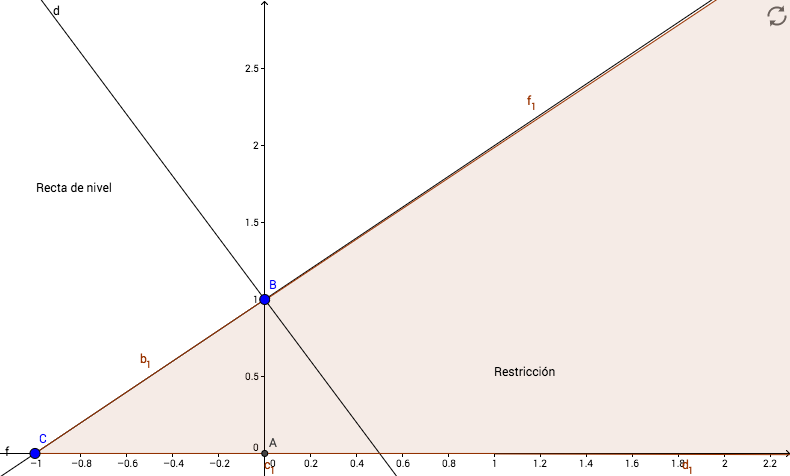
\includegraphics[scale=0.45]{img/io-intro_3.png}
\end{center}

Este problema no tiene una solución óptima.
\end{example}


Vamos a ver otro ejemplo, el \concept{Problema\IS del transporte}
\begin{example}
Trasladar el producto desde donde se produce ($O_i$) hasta donde se demanda ($D_j$) minimizando el coste. 
Cada $O_i$ produce una cantidad determinada $s_i$ y cada centro de demanda consume otra cantidad determinada $d_j$.
Además, $\sum s_i = \sum d_i$.
El coste de traslado desde $O_i$ hasta $D_j$, es $c_{ij}$. 

El problema es determinar qué cantidades hay que trasladar desde $i$ hasta $j$ de forma que se minimice el coste total del transporte.


Vamos a plantear el problema. Vamos a escribir la función objetivo, utilizando $x_{ij}$ como la cantidada que se transporta desde $O_i$ hasta $D_j$

\begin{ioprob}
\goal{$\displaystyle\min \sum_i \sum_j c_{ij}x_{ij}$}
\restrictions{$x_{ij} \geq 0$}{$\displaystyle\sum_j x_{ij} = s_i$}{$\displaystyle\sum_i x_{ij} = d_j$}{}{}{}
\end{ioprob}

Aunque el algoritmo simplex que veremos lo resuelve, la estructura especial del problema hace posible la generación de algoritmos más eficientes. 
Podríamos pensar en la red eléctrica en la que hay del orden de miles de productores y de miles de centrales consumidoras. 
Minimizar costes es importante.
\end{example}

Vamos a ver otro ejemplo más, el \concept{Problema\IS de asignación}
\begin{example}
Hay que asignar n tareas a n trabajadores. Si se asigna la tarea $i$ al
trabajador $j$ se incurre en un coste de $c_{ij}$.
El problema es asignar las tareas a los trabajadores de manera que se minimice el coste.

Podemos darnos cuenta que es el problema del transporte con las restrcciones $s_i = 1$ y $d_j = 1 ∀ij$

Las variables de decisión son:

\[x_{ij} = \left\{ \begin{array}{cc} 1, & \text{ se asigna i al trabajador j}\\0, & \text{ caso contrario}\end{array} \right. \]

\begin{ioprob}
\goal{$\displaystyle\min \sum_i \sum_j c_{ij} x_{ij}$}
\restrictions{$\displaystyle\sum_j x_{ij} = 1$}{$\displaystyle\sum_i x_{ij} = 1$}{$x_{ij}\in\{0,1\}$}{}{}{}
\end{ioprob}

\end{example}


Estos ejemplos son problemas lineales que modelan flujos de transporte en redes, que es lo que veremos a continuación.

\section{Flujo de coste mínimo de una red}

Se considera una red con $n$ nodos $i=1,...,n$ en el que cada nodo tiene una oferta $b_i > 0$ (demanda si $b_i < 0$). 
Suponemos que la red está equilibrada, es decir: $\sum b_i = 0$ y que cada arco tiene un coste $c_{ij}$.

\paragraph{Problema} determinar el flujo $x_{ij}\geq 0$ de coste mínimo tal que el flujo neto en cada nodo sea $b_i$.

Queremos minimizar \[\sum_i \sum_j c_{ij}x_{ij}\]

Con las siguientes restricciones:

\begin{itemize}
	\item $\displaystyle \sum_j x_{ij} - \sum_i x_{ji} = b_i$ Lo que entra en un nodo menos lo que sale tiene que ser igual que la oferta/demanda del nodo. 
	Podemos escribirlo \textbf{matricialmente} tomando $Ax = b$ siendo $A$ la matriz de coeficientes
	\item $x \geq 0$
	\subitem \textbf{Notación: } siendo $x$ un vector, $x > 0$ significa $∀i, x_i>0$. Es interesante darse cuenta que $x \not\geq 0 $ no es equivalente a $x<0$
\end{itemize}


Se plantea el siguiente problema. ¿Dónde queda la restricción de que 2 nodos de la red no estén conectados? Porque en las restricciones definidas no hay nada. 
Una posible solución sería tomar $c_{ij} = \infty$ cuando los nodos no están conectados (práctica habitual en teoría de grafos), aunque computacionalmente, $\infty$ a veces no se puede utilizar como tal. 


\section{Formalización de problemas en general}

\subsection{Forma estándar}

\begin{defn}[Forma\IS estándar de un problema]
Un problema lineal está escrito en forma estándar si es de la forma:
\begin{ioprob}
\goal{$\min c_1x_1 +\cdots +  c_nx_n$}
\restrictions{$a_{11}x_1+\cdots + a_{1n}x_n = b_1$}{$\cdots$}{$a_{m1}x_1+\cdots + a_{mn}x_n = b_m$}{$x_1\geq 0,\ \cdots, x_n\geq 0$}{}{}
\end{ioprob}

Matricialmente, utilizando una matriz $A$ convenientemente podemos escribir:

\begin{ioprob}
\goal{$\min c^\top x$}
\restrictions{$Ax=b$}{$x\geq 0$}{}{}{}{}
\end{ioprob}

\end{defn}

A continuación, vamos a ver una serie de pistas para la formalización de problemas de manera estándar.

\begin{itemize}
	\item Maximizar $f$ es lo mismo que minimizar $-f$.
	\item Si una restricción es: \[\sum_i a_{ji}x_i \leq b_j\] podemos tomar una \concept{variable de holgura}, de tal manera que:
	\[\left(\sum_i^n a_{ji}x_i\right) + x_{n+1} = b_j\]

	¿Y cómo sabemos que esta restricción nos da la misma solución del problema? Vamos a verlo:

	\begin{proof}
		Sea $\gor{x}$ la solución del problema con la restricción con desigualdad.

		Supongamos que existe $x'$ que es mejor que $\gor{x}$ para $(P)$

		$x'$ es factible para $(P)$ implica que $Ax'\leq b \wedge x'\geq 0$. 

		Entonces, $(x',x'_n)$ es mejor que $(\gor{x},\gor{x}_n)$ para $(PE)$, porque:
		\[c^tx'<c^t\gor{x}\]
		\[Ax'+Ix'_n = b\]
		\[x'\geq 0 \wedge \gor{x}\geq 0\]

		Pero habíamos supuesto que $\gor{x}$ es la solución del problema, y hemos visto que si al añadir una variable de holgura no podemos obtener una mejor.
	\end{proof}
	\item Si una restricción es: \[\sum_i a_{ji}x_i \leq b_j\] entonces multiplicamos todo por $-1$
	\item Si una variable $x_i$ no está restringida a tomar valores positivos, se expresa como diferencia de dos variables positivas, es decir:\[x=x'−x'', x'≥0,x''≥0\]

\end{itemize}



\begin{example} Vamos a ver unos cuantos ejemplos de pasar a forma estándar un problema.

\paragraph{Ejemplo 1:\\}

\begin{ioprob}
\goal{$\max3x_1 + 2x_3$}
\restrictions{$x_1 + x_2 + x_3 \leq 1$}{$x_1 - x_2 \leq 5$}{$x_1,x_2,x_3 > 0$}{}{}{}
\end{ioprob}


Para pasarlo a forma estándar, utilizamos las 4 pistas anteriores:\\
\begin{ioprob}
\goal{$\min -3x_1 - 2x_3$}
\restrictions{$x_1+x_2+x_3+x_4 = 1$}{$x_1-x_2+x_5 = 5$}{$x_i \geq 0$}{}{}{}
\end{ioprob}



\paragraph{Ejemplo 2:\\} 

\begin{ioprob}
\goal{$\min 2x_1 + x_2$}
\restrictions{$x_1 - 2x_2 = 0$}{$x_2 \geq 1$}{$x_1$ no tiene restricción.}{}{}{}
\end{ioprob}

Para pasarlo a forma estándar, utilizamos las 4 pistas anteriores:

\begin{ioprob}
\restrictions{$x_1 - 2x_2 = 0$}{$x_2 \geq 1 \to x_2 - x_5 = 1$}{$x_1 = x_3 - x_4$}{$x_3,x_4,x_5 \geq 0$}{}{}
\end{ioprob}

Entonces, queremos minimizar: $(x_3 - x_4) + 2x_2$

\begin{ioprob}
\goal{$\min 2x_1 + x_2$}
\restrictions{$x_1 - 2x_2 = 0$}{$x_2 \geq 1 \to x_2 - x_5 = 1$}{$x_1 = x_3 - x_4$, $x_3,x_4,x_5 \geq 0$}{}{}{}
\end{ioprob}

\paragraph{Ejemplo 3:\\}

\begin{ioprob}
\goal{$\min x_1 + 4x_2+x_3$}
\restrictions{$2x_1 - 2x_2 + x_3 = 4$}{$x_1 - x_3 = 1$}{$x_2\geq 0, x_3\geq 0$}{}{}{}
\end{ioprob}

Para pasarlo a forma estándar, utilizamos las 4 pistas anteriores. 

Necesitamos $x_1 = x_4 - x_5$ con $x_4,x_5\geq 0$ para poder. Reescribimos las restricciones y el objetivo:

\begin{ioprob}
\goal{$\min (x_4 - x_5) + 4x_2 + x_3$}
\restrictions{$x_i\geq 0\, ∀i = 2,3,4,5$}{$2(x_4-x_5) - 2x_2 + x_3 = 4$}{$x_1-x_3 =1$}{}{}{}
\end{ioprob}

\end{example}


\subsection{Forma canónica}

\begin{defn}[Forma\IS canónica de un problema]
Un problema lineal está escrito en forma estándar si es de la forma:


Para problemas de \textbf{minimización}:

\begin{ioprob}
\goal{$\min c^\top x$}
\restrictions{$Ax \geq b$}{$x\geq 0$}{}{}{}{}
\end{ioprob}


 
Para problemas de \textbf{maximización}:

\begin{ioprob}
\goal{$\max c^\top x$}
\restrictions{$Ax \leq b$}{$x\geq 0$}{}{}{}{}
\end{ioprob}

\end{defn}


\section{Problemas de optimización convexos}

\begin{defn}[Problema\IS convexo]
\label{defn:problema_convexo}
Problemas de \textbf{minimización} en los que la función objetivo es convexa, las funciones que definen las restricciones de desigualdad también son convexas y las restricciones de igualdad son lineales. 

Si el problema es de maximización, para que el problema sea convexo la función objetivo debe ser cóncava.
\end{defn}

Una manera de escribirlo formalmente (aunque no todos los problemas convexos estarán escritos exactamente de esta manera) sería
\begin{ioprob}
\goal{$\min f(x)$}
\restrictions{$f_i(x)\leq 0,\,i=1,\ldots,m$}{$a^\top_i x = b_i,\,i=1,\ldots,p$}{}{}{}
donde las funciones $f,f_1,\ldots, f_n$ son convexas.
\end{ioprob}


\begin{example}

Un inversor quiere decidir qué proporción  $x_i$ de los fondos disponibles invierte
en $n$ posibles acciones cuyos beneficios $r_i$, con $i=1,\ldots,n$, son variables aleatorias tales que $\mathbb{E}(r_i)=\mu_i$, $\mbox{Var}(r_i)=\sigma^2_i$ y 
\[
\mbox{Cov}(r_i,r_j) = \sigma_{ij} = \mathbb{E}[(r_i-\mu_i)(r_j-\mu_j)], \ \ i,j=1,\ldots, n.
\]
El beneficio obtenido es $R=\sum_{i=1}^n x_ir_i$.


\

\textbf{Beneficio esperado:} 
\[
\mathbb{E}(R)=\sum_{i=1}^n x_i\mu_i := x^\top \mu.
\]

\

\textbf{Varianza (riesgo) del beneficio:}
\[
\mbox{Var}(R) = \sum_{i=1}^n \sum_{j=1}^n x_ix_j\sigma_{ij} = x^\top\Sigma x.
\]

El objetivo general es maximizar el beneficio con el menor riesgo posible.

\

Un posible problema a resolver para encontrar la cartera óptima:
\begin{ioprob}
\goal{$\max x^\top\mu - \lambda x^\top\Sigma x$}
\restrictions{$\sum_{i=1}^n x_i=1$}{$x\geq 0$}{}{}{}{}
donde $\lambda>0$ es un parámetro que refleja la aversión al riesgo.
\end{ioprob}

Como $\Sigma$ es semidefinida positiva, puede demostrarse que la función objetivo es cóncava, mientras que las restricciones son lineales. Se trata de un \textbf{problema de optimización convexo} (cuadrático).


\end{example}

